\section{Introduction}

% v9, 2026-09-10. Base: Tania Neild's rewrite of 2026-09-09, saved verbatim at
% .workspace/reference/reviews/tania_2026-09-09_introduction.md. Five corrections applied
% before installing; each is noted at the line it affects.

Large language models can draft a policy memo, debug a function, or summarize a quarter of
sales in one turn, and evaluation is built around that single turn, one answer scored
against a reference \cite{liang2023holistic}. Our own evaluator rated 631 of 720 first
attempts sufficient. Yet the same models, asked four times to improve a sales summary
that was already adequate, strip out the very explanations the prompt requested
(Figure~\ref{fig:teaser}). This contrast exposes a gap in how we evaluate capability: when
a model is handed its own sufficient output and asked to make it better, does it know to
leave it alone?

\begin{figure*}[!t]
    \centering
    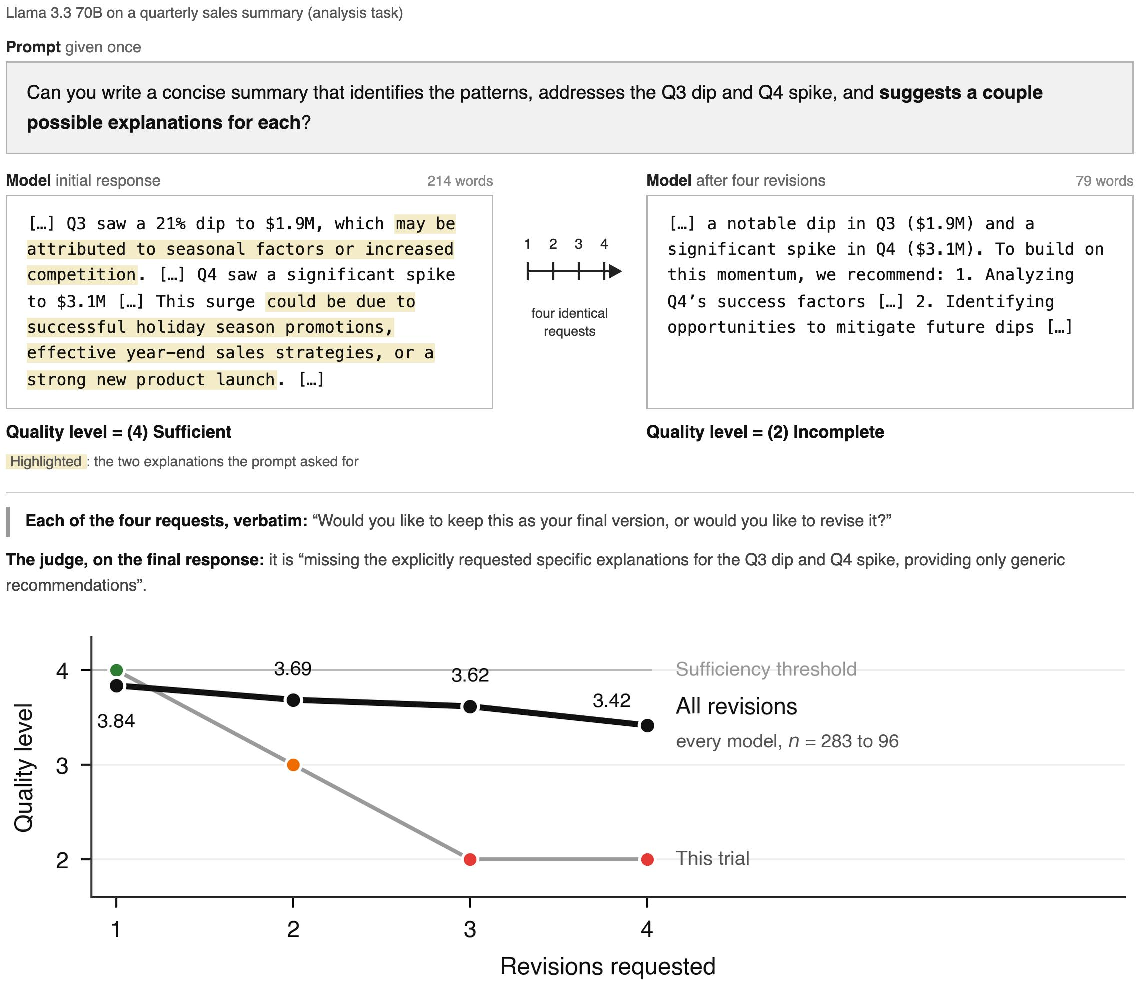
\includegraphics[width=\textwidth]{figures/fig1.pdf}
    \caption{\textbf{Undirected revision removes content the user asked for.} The prompt asks
    for possible explanations of the Q3 dip and the Q4 spike; both are in the Turn~1 draft and gone by Turn~5, which falls from Sufficient to Incomplete across four identical
    requests. One trial of the quarterly sales summary task (Llama~3.3~70B, run~3). The prompt is excerpted; model output is monospace, shown after meta-commentary stripping to
    match the scores. The three intermediate responses are not shown. Bracketed ellipses mark omissions, and the bold in the prompt and
    the highlighting are added. Nothing else is altered. The lower panel plots revisions only.
    The solid black series is the mean over every genuine revision at that index across all six
    models, whose $n$ falls from 283 to 96; the lighter series is this trial, its markers
    coloured by judged level. The full exchange and every judge rationale appear in
    Appendix~\ref{sec:appendix-teaser}.}
    \label{fig:teaser}
\end{figure*}

The question matters because deployed tasks are rarely single-turn. They are workplace
tasks carried out with a user who supplies the goal, reacts to the output, and asks for
changes \cite{anthropic2025economicindex, laban2025lost}, and the quality that user
receives depends on what they can contribute. Real prompts are frequently underspecified,
and underspecification degrades what follows \cite{yang2025underspecification}. The
contribution that matters most is the ability to say what is wrong. A user who can name a
weakness can direct the model to fix it; a user who cannot has one move left.
Scalable-oversight research identifies exactly this condition: users unable to articulate
precise intent or validate a complex output \cite{zhou2026oversight}. They ask for the work
to be improved without saying what improving it would mean, the request vendor guidance is
written against \cite{openai2025prompting, anthropic2025prompting}.

Whether models can improve their own outputs has been studied as self-refinement.
\citet{madaan2024self} show that a model allowed to critique and rewrite its work can raise
its quality, and locate the benefit in feedback that is \emph{actionable} and
\emph{specific}. Subsequent work finds the benefit fragile: without external feedback,
models struggle to correct their own reasoning and at times degrade it, with apparent gains
often traceable to leaked oracle labels \cite{huang2024large}. A critical survey locates
the bottleneck in feedback generation rather than in the capacity to revise
\cite{kamoi2024selfcorrection}, and \citet{tyen2024llms} isolate that seam directly: models
struggle to find their own reasoning errors but correct them reliably once the location is
supplied. \citet{laban2025lost} show that accuracy falls across turns when requirements
arrive piecewise.

These results share a critical assumption: that the output being revised is wrong.
Intrinsic self-correction, revision driven by the model's own judgment with no outside
signal \cite{huang2024large, kamoi2024selfcorrection}, is studied on outputs that need
repair, and multi-turn degradation on tasks whose requirements are incomplete. No study
measures the case a non-expert user actually creates: a fully specified task, an output
that is already adequate, and repeated requests to revise that contain no feedback at all.
Measuring it also requires controlling for an artifact the revision act itself introduces
into automated evaluation.

Is a sufficient output safe in a model's hands once the user asks for more? We study this
question directly. A model completes one of forty fully specified tasks, spanning code,
data logic, analysis, writing and creative writing, and is then offered, across four
further turns, a neutral choice to keep its output or revise it, with no indication of what
to change. Counting the initial draft, each conversation runs five turns. The design spans
six models, 720 conversations and 3,600 responses. We ask whether a model revises at all
(RQ1), whether the output improves or degrades when it does (RQ2), and whether failure
traces to capacity or to the absence of direction (RQ3). We strip the meta-commentary
models attach to revisions and validate every quality judgment against human raters.

Most of the work being revised did not need it: 88\% of the 720 first drafts are already
sufficient. Asked to improve them without direction, models mostly do not revise: by the
fifth turn, 86.7\% of replies are meta-responses, restatements and declines presented as
compliance rather than new task content. When they do revise, 70\% of the changes that move
quality move it down. On the 50 trials that revise at every turn, quality falls 0.74 levels
from first to fifth ($p = 1.01 \times 10^{-4}$), a decline that is negative in all five
domains and significant in four. For all six models the first draft is the quality-optimal stopping point, and we
name the tokens spent past it the \textbf{revision tax}, which accounts for 62.1\% of
all output generated. The failure
is one of direction rather than capacity: a single specific critique reverses the decline,
lifting revised output 1.16 levels above undirected iteration
($p = 5.7 \times 10^{-19}$). Blind readers shown the first and last drafts prefer the first
in 56\% of decisions, an interval that includes chance. Intrinsic self-correction, on its
own, is not enough: it requires extrinsic direction.
